\documentclass[xcolor=dvipsnames]{beamer}
%[xcolor=dvipsnames]
%\usetheme{default}
%\usetheme{default}
\usetheme{Madrid}
\usecolortheme[named=Blue]{structure}
\usepackage{graphicx}
\usepackage{graphics}
\usepackage{epsfig}
%\usepackage{pdfpages}
\usepackage{amsmath,amssymb,multicol}
\usepackage{subfigure}
\newcommand{\blue}[1]{{\color{blue} #1}}
\newcommand{\red}[1]{{\color{red} #1}}
\newcommand{\normal}{\mathcal{N}}
\newcommand{\bc}{\begin{center}}
\newcommand{\ec}{\end{center}}
\newcommand{\bi}{\begin{itemize}}
\newcommand{\ei}{\end{itemize}} \setbeamercovered{transparent}

\graphicspath{{images/}}


\title[Intro Big Data]{Introducing Very Large Data Sets into the Classroom}
\author[D. Kurkiewicz]{Dason Kurkiewicz}
\date{March 9, 2012}
\institute[Stats, ISU]{Department of Statistics, Iowa State University}


\begin{document}

\begin{frame}
\titlepage
\end{frame}


\begin{frame}
  \frametitle{Outline}
  \begin{itemize}
    \pause
      \item Dason's Introduction
    \pause
      \item The GUI
    \pause
      \item The Usability Study
    \pause
      \item Future Work
    \pause
      \item Conclusions
  \end{itemize}
\end{frame}

\begin{frame}
  \frametitle{Introduction}
  \framesubtitle{Meet Dason}


	\begin{figure}[htbp] %  figure placement: here, top, bottom, or page
	   \centering
	   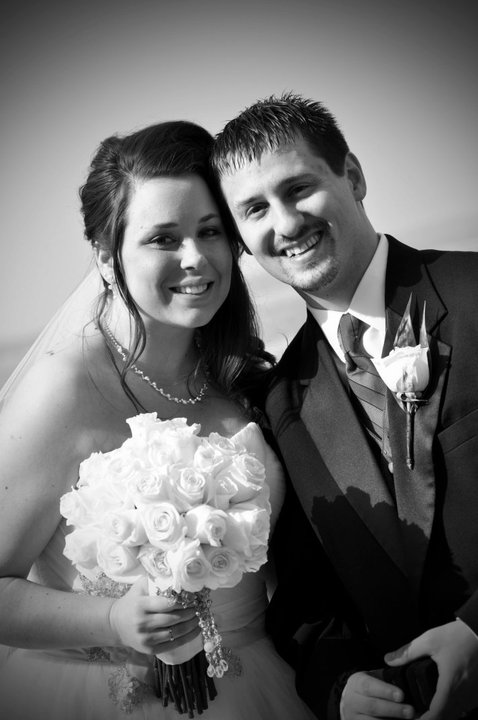
\includegraphics[width=.35\linewidth]{./images/Married.jpg}
        \hspace{.05\linewidth} 
        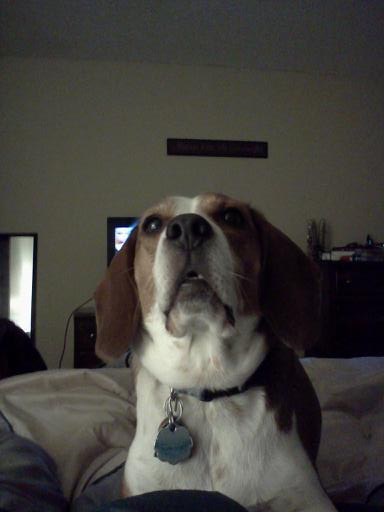
\includegraphics[width=.35\linewidth]{./images/Brutus.jpg}
	   \label{LifePics}
	\end{figure}

	\begin{center}
		My Family
	\end{center}
\end{frame}

%\begin{frame}
%  \frametitle{TISE paper}
%
%  \begin{itemize}
%  
%  \item Submitted paper in January 2011
%  \item Reject May 2011 :(
%  
%
%\end{frame}

\begin{frame}[fragile]
  \frametitle{dbConnectGUI}
  \framesubtitle{Installation}

\begin{verbatim}
# install.packages("gWidgetsRGtk2")
# install.packages("DBI")
# install.packages("RMySQL")

install.packages("dbConnectGUI")
library(dbConnectGUI)
# Try it out
dbConnectGUI()
# Or
connect <- getConnection()
dbConnectGUI(connect$con)
\end{verbatim}


\end{frame}


\begin{frame}
  \frametitle{dbConnectGUI}
  \framesubtitle{Connection Dialog}
  \centering
  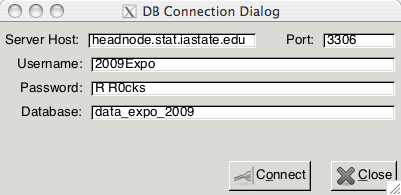
\includegraphics[width=.70\linewidth]{./images/dbconnect-dialog.png}

\end{frame}

\begin{frame}
  \frametitle{dbConnectGUI}
  \framesubtitle{Data Viewer}
  \centering
  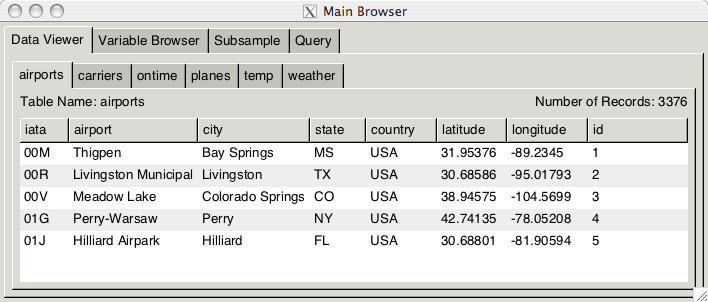
\includegraphics[width=.85\linewidth]{./images/db-lineviewer.png}

\end{frame}

\begin{frame}
  \frametitle{dbConnectGUI}
  \framesubtitle{Variable Browser}
  \centering
  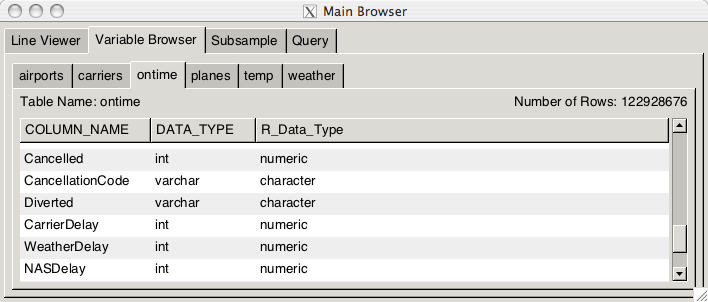
\includegraphics[width=.85\linewidth]{./images/db-variablebrowser.png}

\end{frame}

\begin{frame}
  \frametitle{dbConnectGUI}
  \framesubtitle{Subsample}
  \centering
  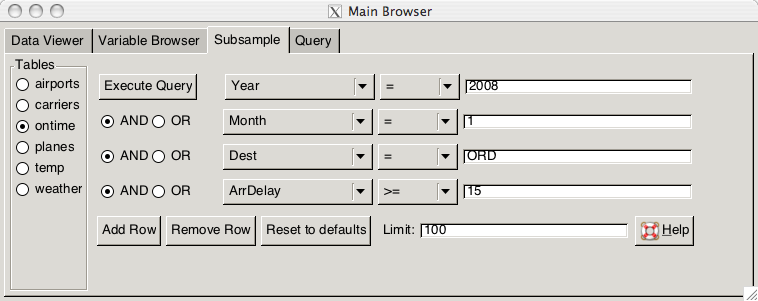
\includegraphics[width=.85\linewidth]{./images/db-sample.png}

\end{frame}

\begin{frame}
  \frametitle{dbConnectGUI}
  \framesubtitle{Query}
  \centering
  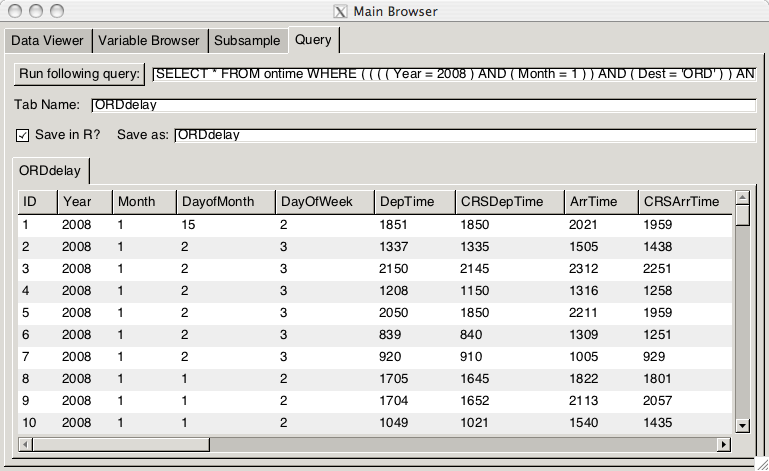
\includegraphics[width=.85\linewidth]{./images/db-query.png}

\end{frame}

\begin{frame}
  \frametitle{dbConnectGUI}
  \framesubtitle{Changes}
  \centering
  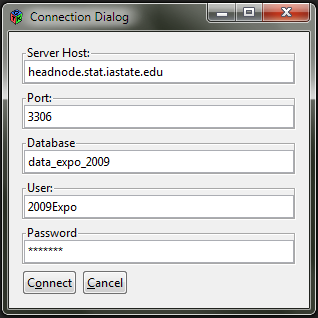
\includegraphics[width=.50\linewidth]{./images/db-ConnectNew.png}

\end{frame}

\begin{frame}
  \frametitle{Learning Objectives}
	
	\begin{itemize}
	\item Familiarizing students with databases and exploring the utility of databases for effcient data storage.
	\item Obtaining access to data stored in databases.
	\item Searching databases for specifc data records of interest as well as learning how to extract such data records for further statistical analysis in R or a different software package.
	\item Providing students with a first gentle and more paced introduction to the SQL language. The GUI can help facilitate the learning process and potentially improve student's attitude toward learning the database language SQL.
	\end{itemize}

\end{frame}

\begin{frame}
  \frametitle{Usability Study}
  \framesubtitle{Student Overview}


	\begin{table}[htbp]
	   \centering
	   \begin{tabular}{lrrrr} 
	      \hline
		  & \multicolumn{2}{c}{400-level} & \multicolumn{2}{c}{500-level}  \\
	      \hline
	      & Statistics & non-Statistics       & Statistics & non-Statistics \\
	       \hline
	      Undergraduate & 23 & 6 & 1 & 0 \\
	      Graduate & 1 & 8 & 21 & 15 \\
	      \hline
	   \end{tabular}
	   \caption{Overview of students participating in the usability study by course, status, and area.}
	   \label{fb-overview}
	\end{table}
\end{frame}

\begin{frame}
  \frametitle{Usability Study}

\begin{figure}[htbp] %  figure placement: here, top, bottom, or page
   \centering
   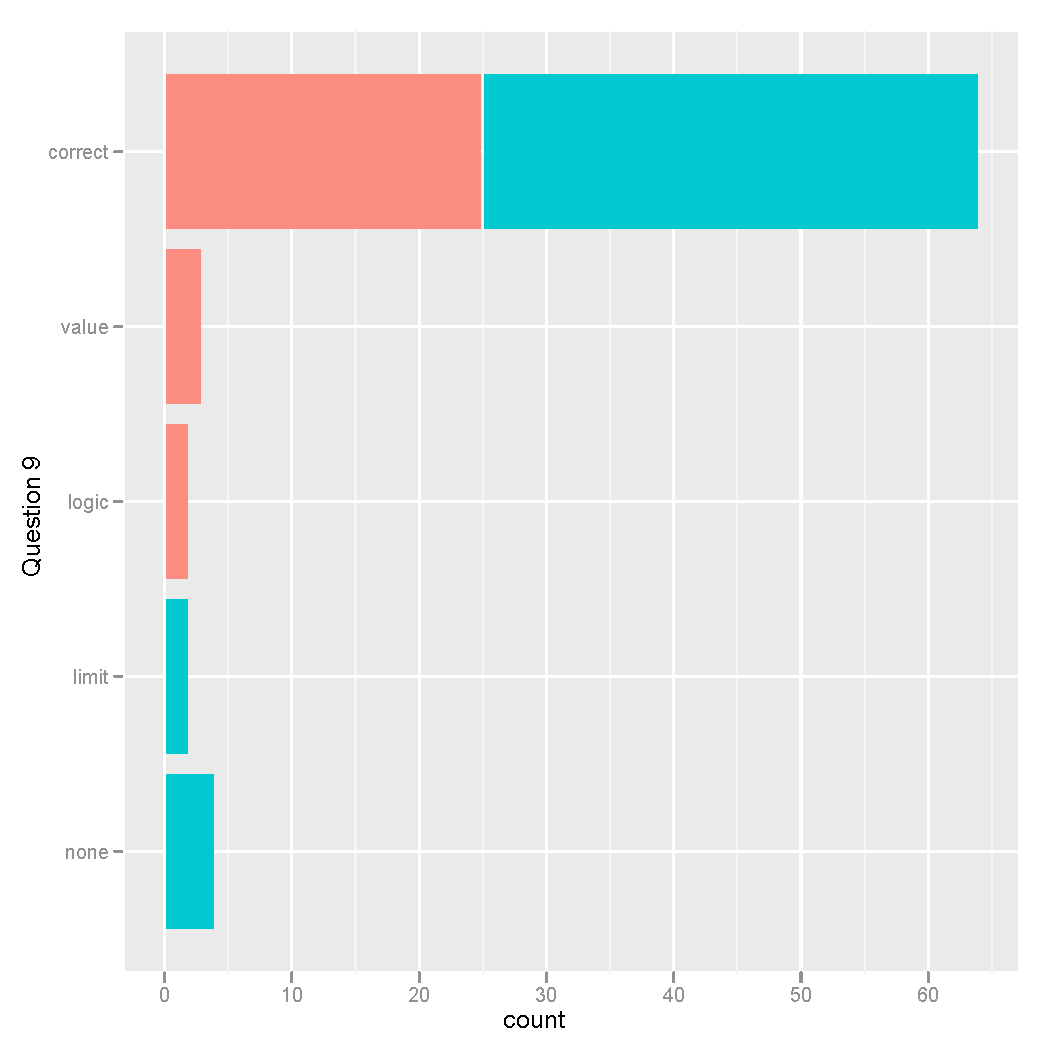
\includegraphics[width=.33\linewidth,  keepaspectratio=true]{fb-question-9.pdf} 
   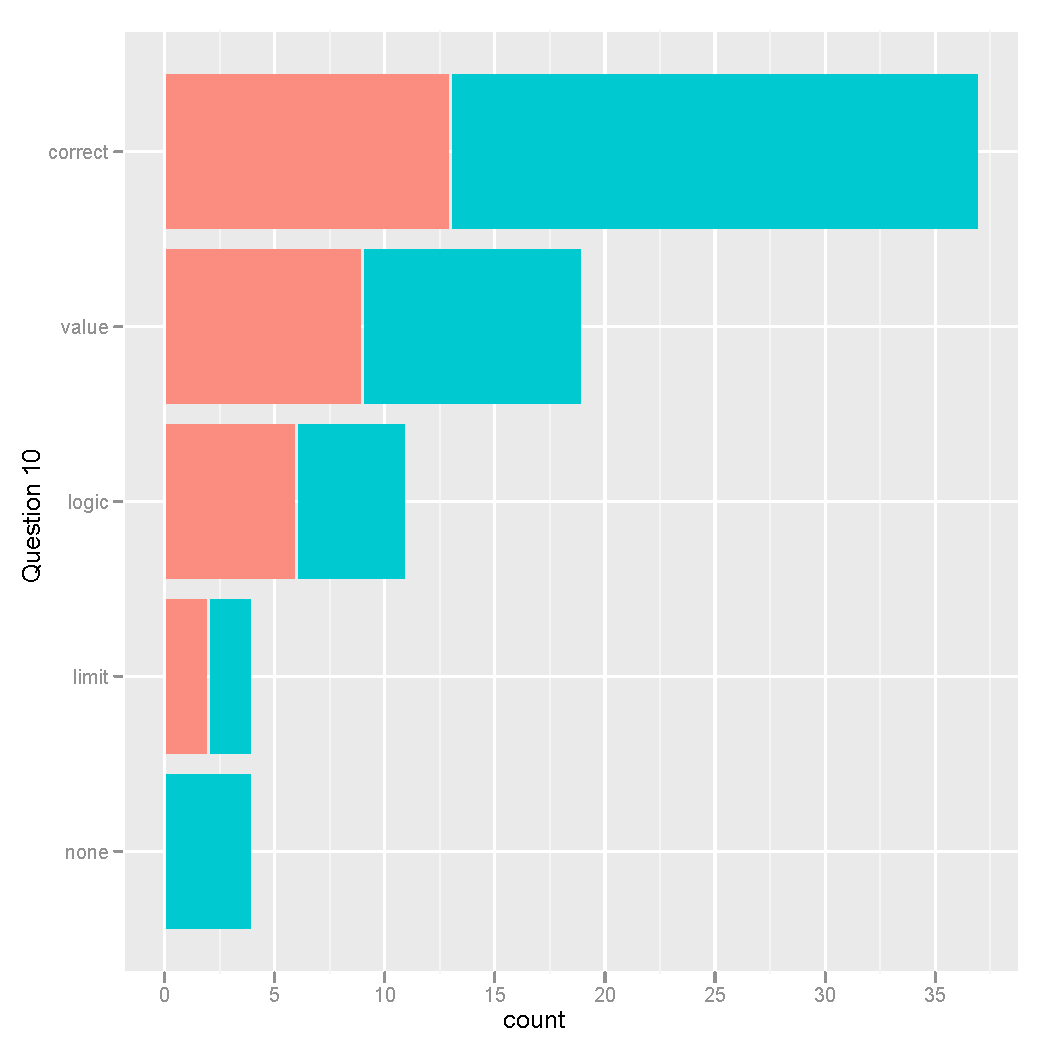
\includegraphics[width=.33\linewidth,  keepaspectratio=true]{fb-question-10.pdf} 
   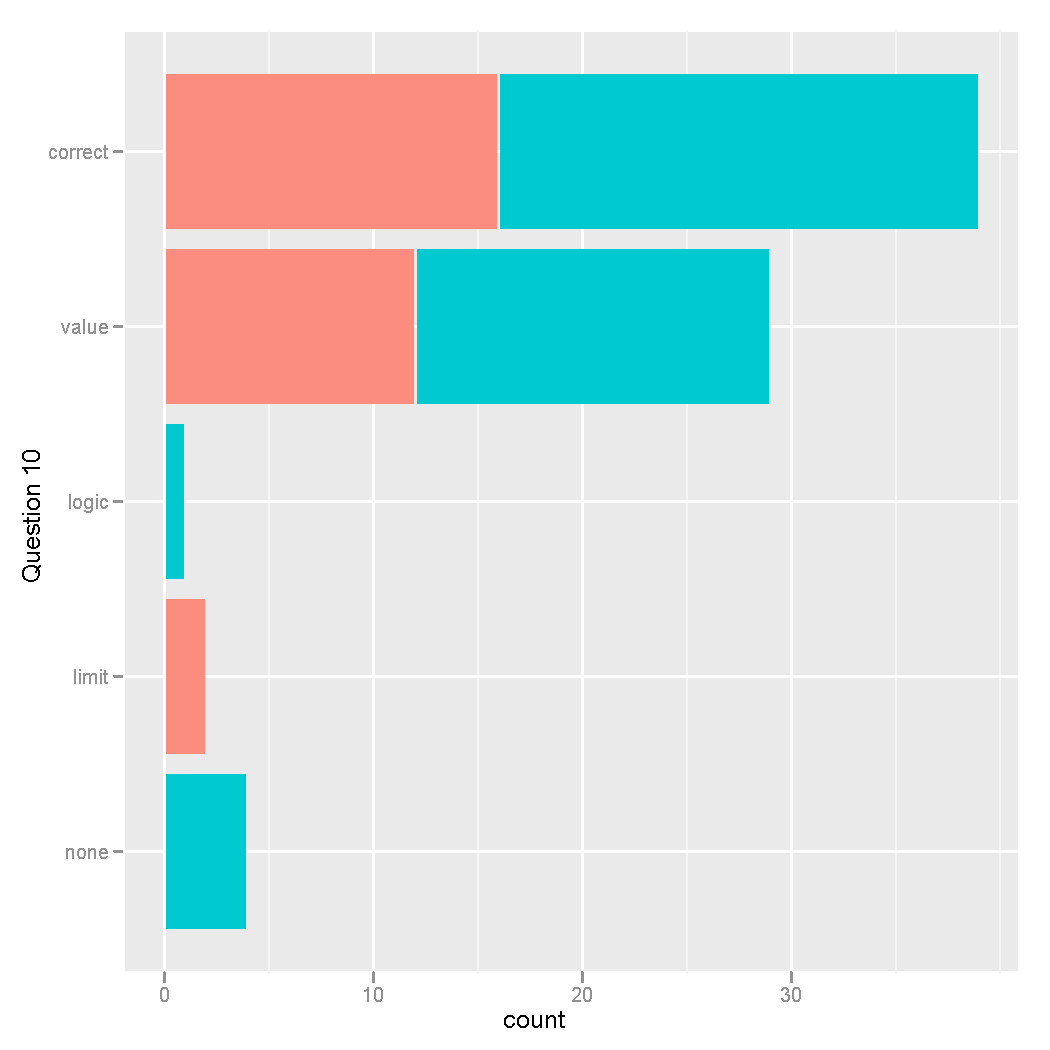
\includegraphics[width=.33\linewidth,  keepaspectratio=true]{fb-question-11.pdf} 
 
   
\includegraphics[height=.25in, keepaspectratio=true]{fb-legend2.pdf} 
   %\caption{Students' feedback on questions 9, 10, and 11. Wrong answers are classified according to source of error. `value' and `logic' can potentially be considered carelessness errors rather than mistakes due to lack of understanding of the GUI. Categories `limit' (specifying a wrong limit of data records) and `none' (not providing any answer) are more serious errors and indicate a lack of understanding of the GUI.} 
   \label{fb-errors}
\end{figure}
\end{frame}

\begin{frame}
  \frametitle{Usability Study}
\begin{figure}[htbp] %  figure placement: here, top, bottom, or page
   \centering
   %\begin{subfigure}
   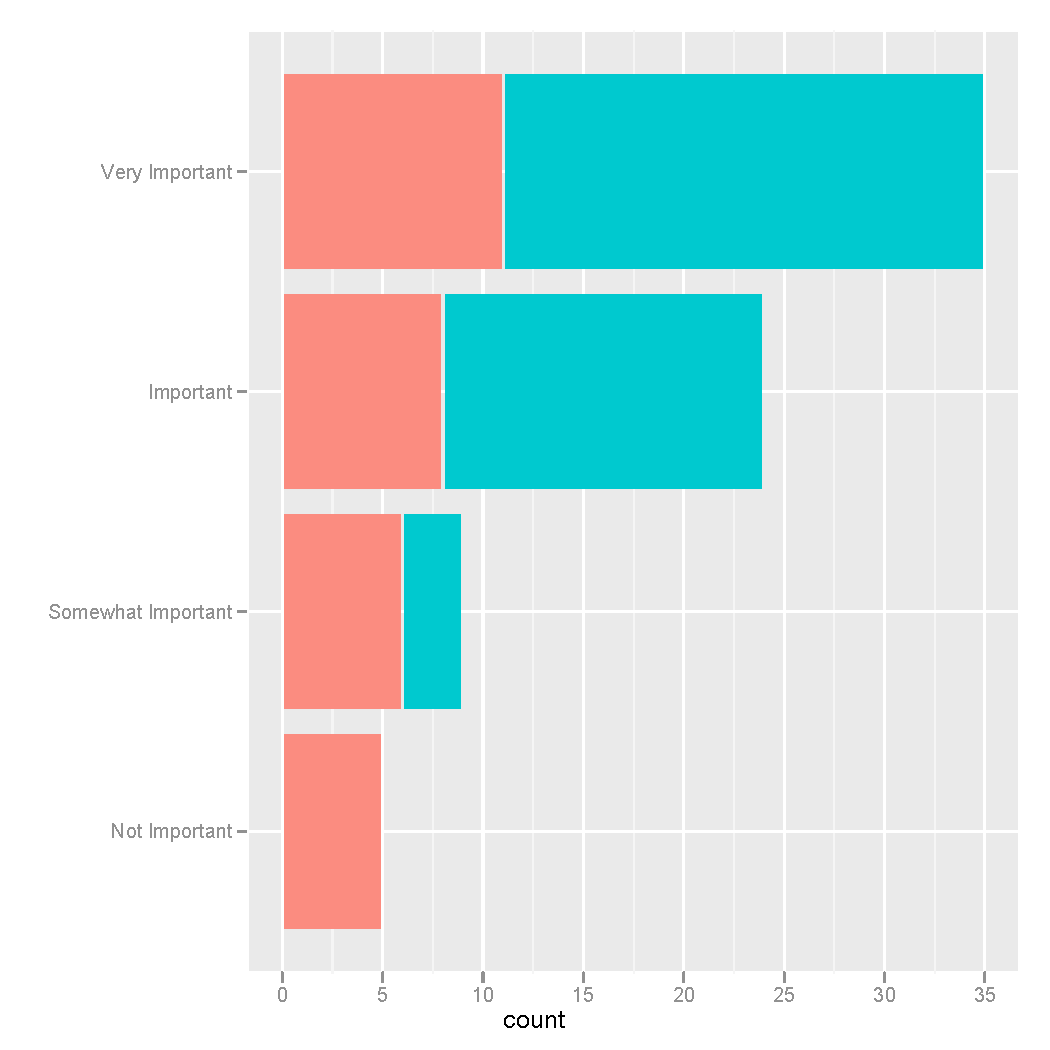
\includegraphics[width=.5\linewidth, keepaspectratio=true]{fb-importance.pdf} 
   %\caption{hey}
   %\end{subfigure}
   %\begin{subfigure}
   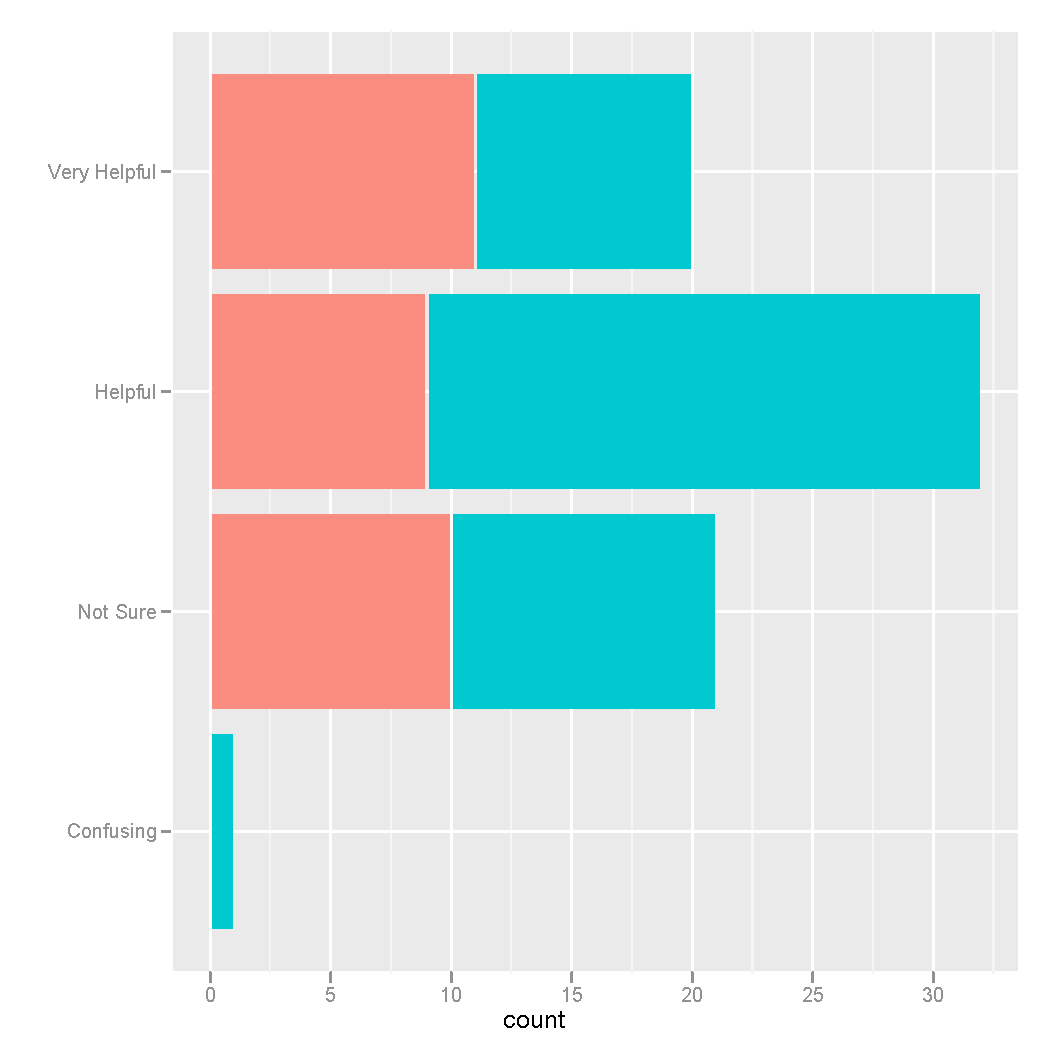
\includegraphics[width=.5\linewidth, keepaspectratio=true]{fb-useful.pdf} 
   %\caption{no}
   %\end{subfigure}
   %
\includegraphics[width=.2\linewidth, keepaspectratio=true]{fb-legend.pdf} 
   \caption{User feedback: perceived importance of task (left) and usefulness of the GUI to help with the task (right). Undergraduates are red and Graduates are Blue.}
   \label{fb-use-importance}
\end{figure}
\end{frame}

\begin{frame}
  \frametitle{Usability Study}
  \framesubtitle{Students' opinions on task difficulty}
\begin{figure}[htbp] %  figure placement: here, top, bottom, or page
   \centering

   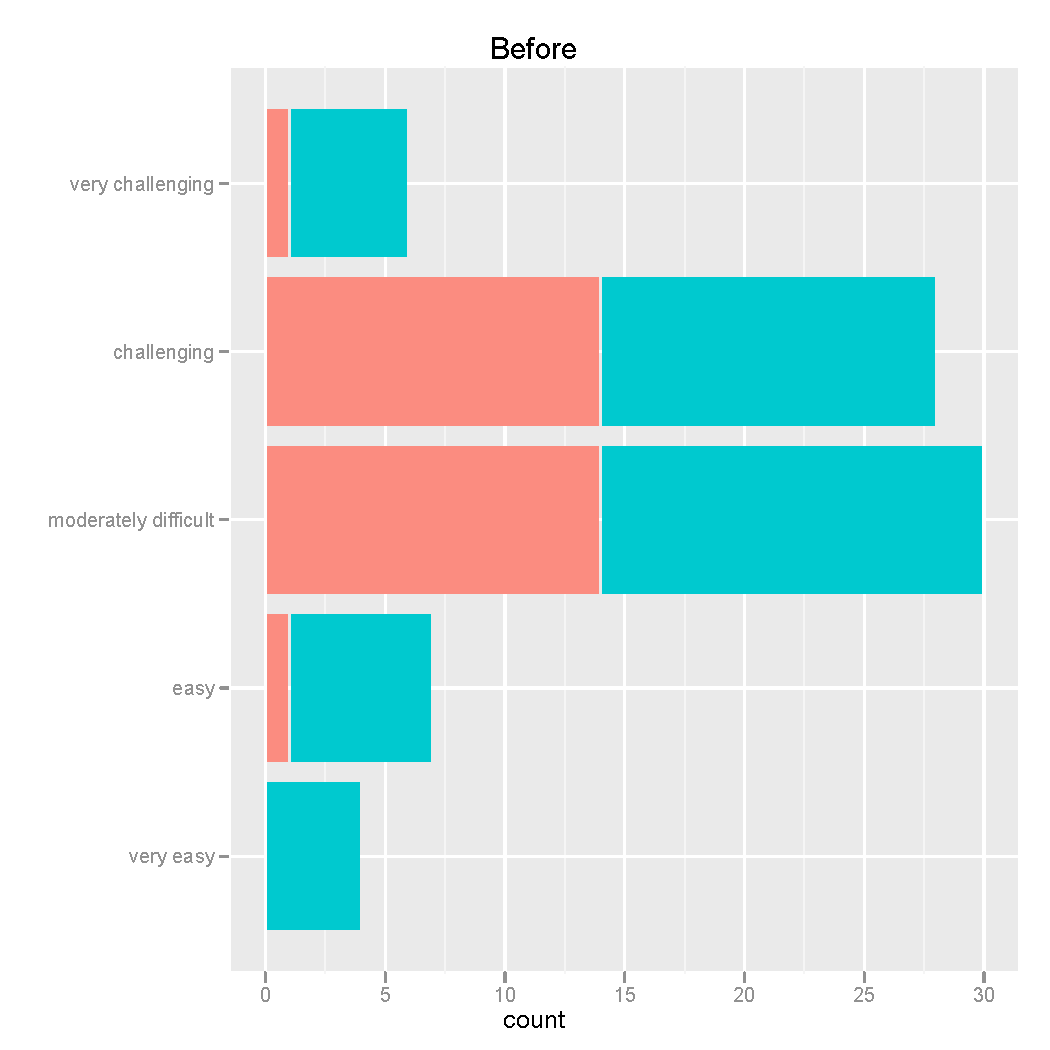
\includegraphics[width=.5\linewidth,  keepaspectratio=true]{fb-before.pdf} 
   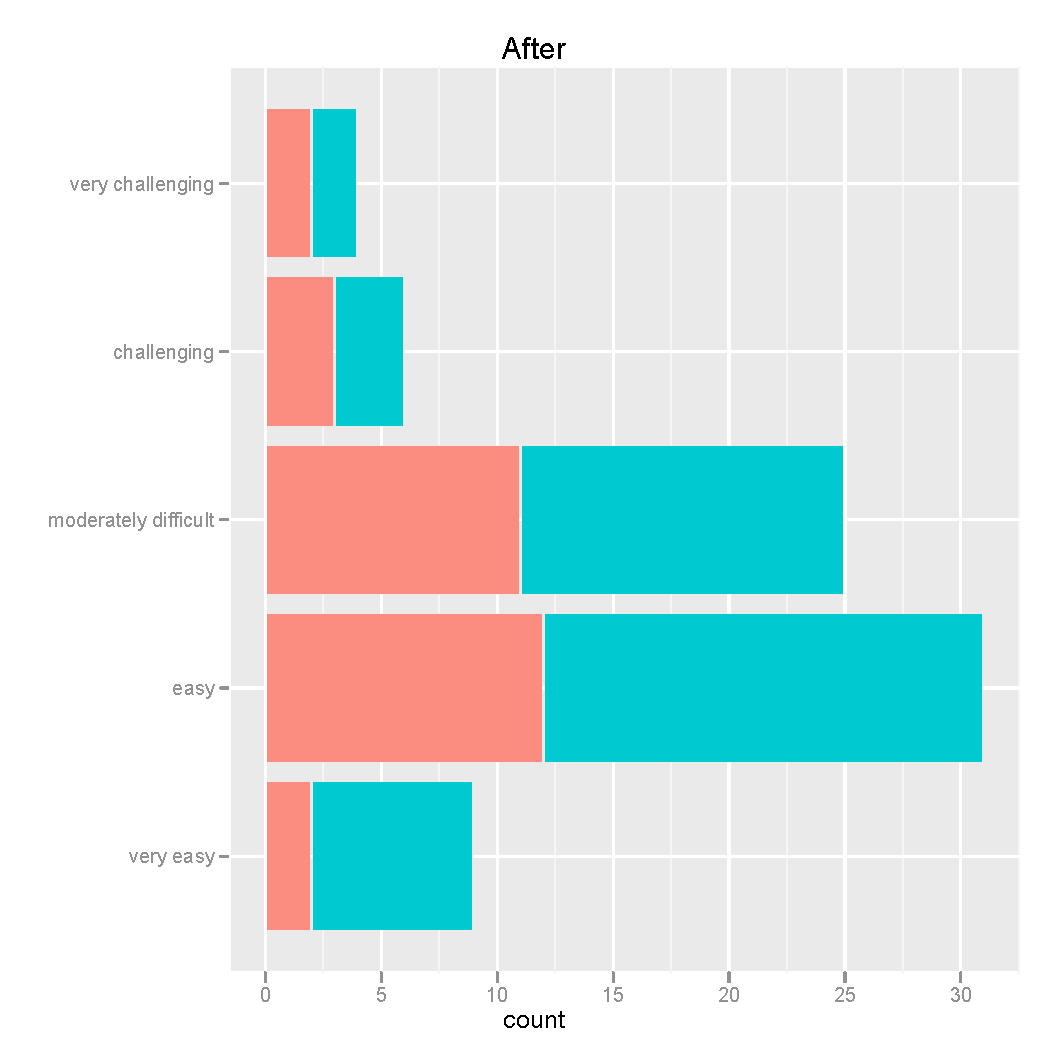
\includegraphics[width=.5\linewidth,  keepaspectratio=true]{fb-after.pdf} 
   %
\includegraphics[height=2in,  keepaspectratio=true]{fb-legend.pdf} 
   \caption{User feedback: anticipated degree of difficulty is greater than experienced difficulty of the task. Undergraduates are Red and Graduates are Blue.}
   \label{fb-before-after}
\end{figure}
\end{frame}


\begin{frame}
  \frametitle{Paired Comparison of Before/After Difficulty}


\begin{figure}[htbp] %  figure placement: here, top, bottom, or page
   \centering
   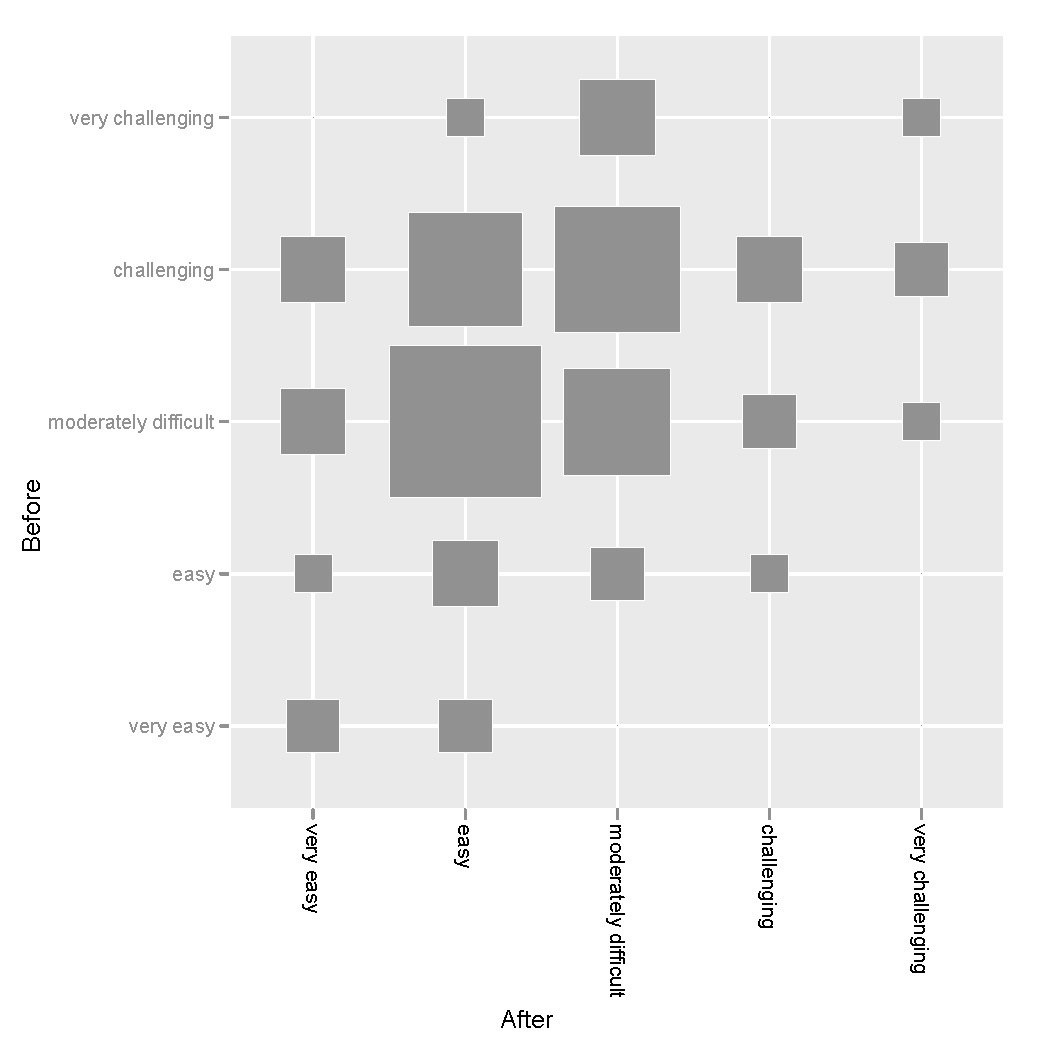
\includegraphics[width=.6\linewidth, keepaspectratio=true]{fb-before-after.pdf} 
   %\caption{Fluctuation diagram of students' assessment of task difficulty before and after completion of  the study. Generally, students find the task easier than they anticipate.}
   \label{fb-before-and-after}
\end{figure}
\end{frame}


\begin{frame}
  \frametitle{Future Work}
  
  \begin{itemize}
    \pause
    \item Efficient Random Stratified Samples
    \pause
    \item Joins
    \pause
    \item Tutorial
  \end{itemize}
\end{frame}

\begin{frame}
  \frametitle{Closing Remarks}
  \begin{itemize}
    \pause
    \item Big data is here to stay
    \pause
    \item GUIs provide a level of comfort to some
    \pause
    \item The usability study shows there is benefit to using the GUI
    \pause
    \item Will keep working to make this better
  \end{itemize}

\end{frame}

\begin{frame}
  \frametitle{The End}
   \centering
   \huge
   Questions?

\end{frame}


\end{document}
